\chapter{Metodologia}\label{cap:metodologia}

Neste capítulo é descrita a sequência de etapas que serão realizadas neste trabalho para que os objetivos de pesquisa sejam alcançados. 

%Iniciaremos com uma revisão bibliográfica para conhecer o estado da arte e depois definir as características que representarão os padrões a serem classificados. Em seguida, faremos um levantamento das classes relevantes para classificação de terrenos neste tipo de imagens aéreas, considerando a relevância destes para a problemática em questão.

%Em um momento posterior será feito um levantamento na literatura sobre algoritmos e métodos comumente usados para a segmentação das imagens por tipo de terreno. Por fim, experimentos serão realizados para identificar os métodos (vetor de características e técnicas de aprendizado) com maior taxa de acurácia para o problema específico de segmentação por tipo de terreno em imagens aéreas da região de floresta amazônica.

A primeira etapa do trabalho é a segmentação das imagens por tipo de terreno. Os métodos de segmentação de imagens considerados estado-da-arte serão aplicados à uma parte da base de imagens aéreas da floresta amazônica. Esta porção da base de imagens será manualmente segmentada por seres humanos e servirá de base de comparação para a segmentação realizada pelos métodos experimentados. Esta etapa deve determinar o método a ser utilizado na solução descrita pelo trabalho.

Posteriormente, as regiões encontradas na segmentação das imagens devem ter suas características extraídas para serem classificadas dentre diversas classes: floresta, vegetação rasteira, clareira, corpos d'água e elementos anômalos. É nesta etapa que se dará o primeiro nível de classificação. Para esta etapa, serão utilizados os métodos descritos na seção \ref{sec:trClassificacao}. Os resultados de cada método serão comparados à uma classificação realizada por seres humanos, permitindo que os métodos de aprendizagem supervisionados sejam utilizados. As regiões classificadas como "elementos anômalos" serão prontamente consideradas objetos de interesse. As demais regiões serão classificadas de acordo com seu tipo de terreno pertinente e serão investigadas com mais detalhes na próxima etapa.

A última etapa de classificação consiste em utilizar modelos de aprendizado específicos para cada tipo de terreno, para detectar objetos de interesse que não foram encontrados na etapa de segmentação, normalmente pequenos demais para serem definidos como uma região \textit{per se}, e que estão contidos em regiões maiores. Cada tipo de terreno possuirá um modelo de classificação específico, podendo se utilizar de um vetor de características diferente dos demais terrenos, para otimizar a precisão na detecção dos objetos de interesse. Nesta etapa, diversos classificadores serão treinados e testados para cada tipo de terreno e seus resultados serão comparados com uma classificação manual feita por seres humanos. Nesta etapa serão explorados classificadores unários e multi-classe a fim de obter o melhor resultado na deteção dos objetos de interesse e um classificador, com seus parâmetros e vetor de características, será selecionado para cada tipo de terreno.

Por fim, unindo a saída do primeiro nível de classificação, onde regiões de "elementos anômalos" podem ser encontradas, com a saída do segundo nível, onde os objetos de interesse serão procurados no interior das demais regiões, teremos uma saída única, apontando as regiões de uma imagem que possuam objetos de interesse na problemática em questão.

As sucessivas validações e comparações com a segmentação manual feita por seres humanos é importante para diminuir o erro em cada etapa, visto que imprecisões em um dos passos tende a propagar o erro nos passos seguintes. Se tomarmos como exemplo o princípio da solução, uma segmentação inadequada de uma imagem pode dificultar o primeiro nível de classificação, responsável pela classificação do tipo de região encontrada.

A arquitetura geral da solução pode ser vista na figura \ref{fig:metDiagrama}.

\begin{figure}[h]
    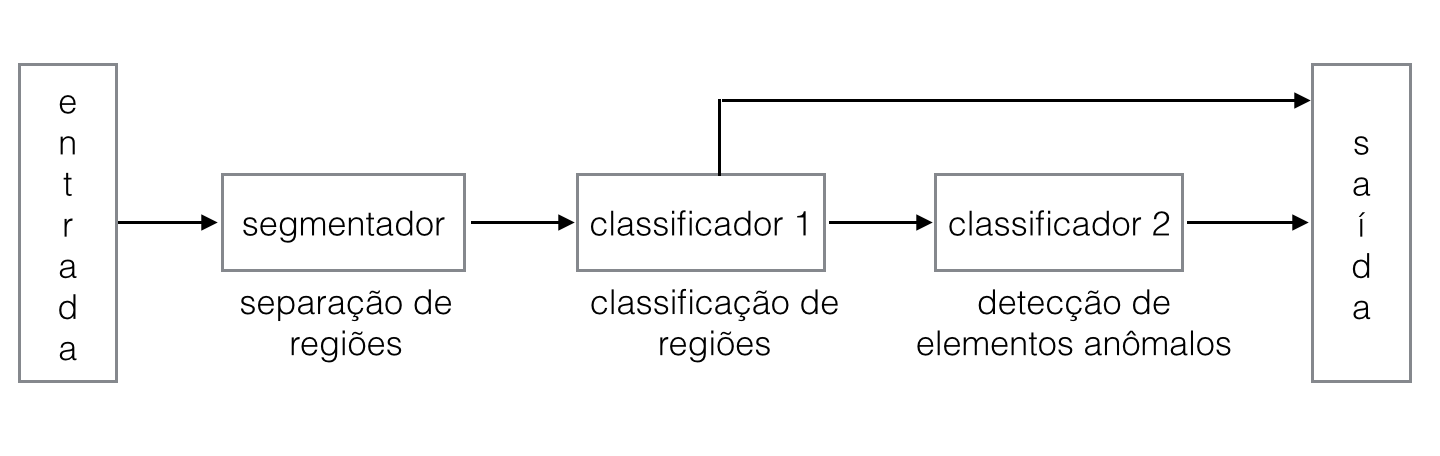
\includegraphics[width=\textwidth]{imgs/arquitetura}
    \caption{Arquitetura da solução a ser desenvolvida para detecção de anomalias em imagens aéreas da floresta amazônica}
    \label{fig:metDiagrama}
\end{figure}

Durante o desenvolvimento do trabalho, artigos serão submetidos com os resultados intermediários, para divulgação e validação junto à comunidade científica. Por fim, a dissertação final do programa de mestrado será redigida, contendo o resultado dos experimentos, seus êxitos e problemas encontrados.